\chapter{Introduction}
\section{Hi!}
First of all, thanks for trying out Little Sound Dj!

A lot of effort has been put into making this program as powerful and fast-worked
as possible. If you don't have previous experience from similar ``tracker"-like
music editors, the amount of new concepts may seem a bit overwhelming at first.
Please, try not to stress about it. Learn step by step, keep it fun and progress
at your own pace. Within days, you should know enough about the
program to make your own first songs.

This manual is mostly written as an absolute beginners guide, but also as a reference
that covers everything in the program. However, there still
is a lot of information that would not fit into a manual like this. I highly recommend
checking out the user-maintained Wiki site at \url{http://wiki.littlesounddj.com} -
it contains material like tutorials, tips and tricks, and
hardware related DIY projects. Also, the Facebook group
at \url{https://www.facebook.com/groups/LittleSoundDJ/} is useful for getting in touch
with other users.
If you have questions or bug reports, please e-mail
\href{mailto:info@littlesounddj.com}{info@littlesounddj.com}.

Happy tracking!

\textit{/Johan}

\section{Important Notice}

Turning off the Game Boy while playing may cause your songs to be lost, so please avoid that.
Also, it is best to avoid using the program when batteries are low enough to risk that the
Game Boy shuts down itself. Low battery level is indicated by the red light on your Game Boy
becoming faint, or the screen becoming dim.

\section{Game Boy Sound}
The Game Boy sound chip has four channels, each with 4-bit resolution.

\begin{description}
\item[Pulse Channel 1] Square wave with envelope and sweep functions.
\item[Pulse Channel 2] Square wave with envelope function.
\item[Wave Channel] Soft synthesizer, sample playback and speech synthesis.
\item[Noise Channel] Noise with envelope and shape functions.
\end{description}


\section{Key Presses}
In this documentation, key presses are marked up in this fashion:
\begin{description}
\item[\textsc{a}] \textsc{a} button
\item[\textsc{b}] \textsc{b} button
\item[\textsc{start}] start button
\item[\textsc{select}] select button
\item[\textsc{left}] left arrow
\item[\textsc{right}] right arrow
\item[\textsc{up}] up arrow
\item[\textsc{down}] down arrow
\item[\textsc{cursor}] pressing any arrow key
\item[\textsc{left/right}] pressing left or right arrow
\item[\textsc{up/down}] pressing up or down arrow
\item[\textsc{select+a}] pressing \textsc{a} while holding \textsc{select}
\item[\textsc{select+(b,b)}] pressing \textsc{b} twice, while holding \textsc{select}
\end{description}

\section{Navigating the Program}
After starting up LSDj, you should be facing a screen like the one in figure~\ref{fig:song}.

\begin{figure}[hbtp]
\centering
\fbox{ 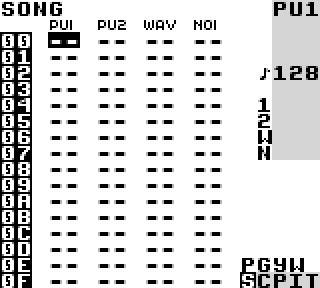
\includegraphics{song} }
\caption{Song Screen}
\label{fig:song}
\end{figure}

The \textsc{song} title at the top left of the window indicates that this is the song screen, the
window where you arrange your songs. The four columns with dashes each represent a
Game Boy sound channel. There are two pulse wave channels, one custom wave channel
(which uses sampled drum kits or soft-synthesized wave forms), and one noise channel. You
can move around between the different channels using the cursor key.
\begin{figure}[hbtp]
\centering
\fbox{ 
\includegraphics{map} }
\caption{Screen Map}
\label{fig:map}
\end{figure}

Little Sound Dj uses several screens, which are laid out on a \begin{math} 5 \times 3 \end{math} map, displayed in the
bottom right of the screen (figure~\ref{fig:map}). The most useful screens are laid out in the middle row, also called
the main row. It contains the song, chain, phrase, instrument and table screens. These screens
are ordered after level detail. The leftmost song screen presents an overview over the entire
song, whereas the rightmost table screen is for detailed instrument programming. You can
navigate between the different screens by holding \textsc{select} and pressing the cursor key.

The song, chain and phrase screens are used for sequencing, and work together in a tree-structure
fashion. The phrase screen is a 16-step sequencer where the actual note data is
entered. The chain screen is a 16-step sequencer where you can enter sequences of phrases to
be played back. The song screen is a 256 step long sequencer, where you enter sequences of
chains to be played back.

\section{Making Your First Sounds}
Navigate to the song screen, and put the cursor on the \textsc{pu1} column. Now tap the \textsc{a} button
twice to insert a new chain. The digit 00 should appear at the cursor. You can now edit chain 0 by pressing \textsc{select+right} and entering the chain screen. There, go through the
same procedure: tap \textsc{a} twice to insert a new phrase, and press \textsc{select+right} to go to the
phrase screen.

\begin{figure}[hbtp]
\centering
\fbox{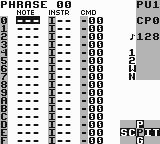
\includegraphics{phrase}}
\caption{Phrase Screen}
\label{fig:phrase1}
\end{figure}

In the phrase screen, you can enter notes to be played back. Move the cursor to the note
column and press \textsc{a} to enter a note. The text C-2 will appear: C being the note, and 3 the
octave. Press \textsc{start} to play back the phrase. Note how the phrase is played back from the
top of the screen to the bottom. You can change the note value by holding \textsc{a} and pressing the
cursor button. \textsc{a+left/right} changes the note, and \textsc{a+up/down} changes octave.

You can now try to move the cursor up and down and insert more notes in other positions. If
you want to delete a note, press \textsc{a} while holding \textsc{b}. When you have finished listening, press
\textsc{start} again to stop the phrase.

The clean pulse sound might get a bit dull after while. Let's move on to the instrument
screen by pressing \textsc{select+right}.

\begin{figure}[hbtp]
\centering
\fbox{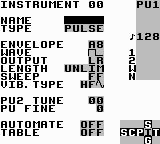
\includegraphics{instr-pulse}}
\caption{Instrument Screen}
\label{fig:instr}
\end{figure}

In the instrument screen, we can make the sound a little bit more interesting. Try to change
the envelope and wave fields by moving the cursor there and pressing \textsc{a+left/right}. Try
to modify the envelope setting from \texttt{A8} to \texttt{A3}. Now, press \textsc{start} again to hear any
change in sound. The sound should now be more bouncy.

The type field sets the instrument type. The instrument types are specific for different
channels -- pulse instruments should only be played back in the pulse channels, wave and kit
instruments in the wave channel, and noise instruments in the noise channel.

Let's try out the sampled drum kits. Now, we have to change channel to the wave channel.
Go back to the song screen, move the cursor over to the wave channel, and create a new
chain and a new phrase the way you did before (tapping \textsc{a} twice on empty steps). Then,
move over to the \textsc{instr} column in the phrase screen, and tap \textsc{a} twice to create a new
instrument. Press \textsc{select+right} to edit that instrument, change the instrument type to
\textsc{kit} by pressing \textsc{a+right} once on the type field, then go back to the phrase screen. Now,
you should be able to enter drum sounds the same way you entered notes before.

\section{Initial Troubleshooting}

Does your cartridge not start, crash, or act strange in other ways? Here are some things to try.

\begin{itemize}
\item Clean cartridge pins using a cotton swab and alcohol.
\item Re-insert the cartridge a couple of times to remove oxide.
\item Make sure that the cartridge is firmly plugged in. Sometimes it can help to put a piece of tape on the cartridge to give it a snug fit.
\item Replace batteries with fresh ones.
\item Do a full reset of the cartridge memory. This is done by pressing \textsc{select+a+b} on the \textsc{load/save file} button in project screen.
\item Search for help on the Little Sound Dj Wiki (\url{http://wiki.littlesounddj.com}) or ask in the Facebook group.
\end{itemize}

\section{Hexadecimal Number System}

Before moving on to the next chapter, now is a good time to get introduced with the hexadecimal number system that Little Sound Dj uses for representing values.

The hexadecimal number system works just the same way as the traditional decimal number system. The only difference is that it's base is 16 instead of 10. This means it consists of 16 unique symbols: the digits 0 to 9, followed by the letters A to F. For clarity, this manual will mark hexadecimal values with a dollar sign.
As an example, let's print a table of numbers -- first with decimal digits, then with
hexadecimal digits\ldots

\begin{figure}[hbtp]
\centering

\begin{tabular}{r|r|r|r|r|r|r|r|r|r|r}
 Decimal & 1 & 2 & 3 & 4 & 5 & 6 & 7 & 8 & 9 & 10 \\
\hline
 Hexadecimal & \$1 & \$2 & \$3 & \$4 & \$5 & \$6 & \$7 & \$8 & \$9 & \$A \\
\end{tabular}

\begin{tabular}{r|r|r|r|r|r|r|r|r|r|r}
 Decimal & 11 & 12 & 13 & 14 & 15 & 16 & 17 & 18 & 19 & 20 \\
\hline
 Hexadecimal & \$B & \$C & \$D & \$E & \$F & \$10 & \$11 & \$12 & \$13 & \$14  \\
\end{tabular}

\end{figure}

Note that the hexadecimal and decimal values are really equal; just the representations differ.
The reason to use the hexadecimal system here is to save screen space; with hexadecimal
numbers, it is possible to represent every byte value using no more than two digits. (The
value range is 0 to 255 -- that is, \$0 to \$FF.)

Representing negative numbers with two digits only can be a problem. In Little Sound Dj,
the numbers are wrapping. That means, when subtracting one from the smallest possible
number (\$0), it will jump to the highest possible value (\$FF). So \$FF can represent -1 as well as 255, depending on the situation.

If you don't get all this immediately -- please don't worry too much -- it will become clear to you as you spend time with the program.



